\documentclass[a4paper,12pt]{article}

%% Definitioner för vågfysikrapporten-dokument

%% Text-kodning, språk samt PS-font
\usepackage[utf8]{inputenc}
\usepackage[T1]{fontenc}
\usepackage{ae,aecompl}
\usepackage{listings}
% % bitmap-grafik
\usepackage{graphicx}
\usepackage{svg}
% % matematik
\usepackage{mathtools}
\usepackage{latexsym}
\usepackage{caption}
\usepackage{subcaption}

%% Paragrafformat
\setlength{\parindent}{0pt}
\setlength{\parskip}{1ex plus 0.5ex minus 0.2ex}

%% Format för datum
\newcommand{\twodigit}[1]{\ifthenelse{#1<10}{0}{}{#1}}
\newcommand{\dagensdatum}{
\number\year-\twodigit{\number\month}-\twodigit{\number\day}}

%% Sidhuvud och sidfot
\usepackage{fancyhdr}
\pagestyle{fancy}
\lhead{Alexander Poole}
\chead{TSDT14}
\rhead{Anna Hjelmberg}
\lfoot{alepo020@student.liu.se}
\cfoot{{\ } \\ \thepage}
\rfoot{annhj876@student.liu.se}


\title{TSDT14 - Report}
\author{Alexander Poole - alepo020 \\ Anna Hjelmberg - annhj876}


%%Dokumentets början
\begin{document}
\maketitle
	\thispagestyle{empty}
\newpage

\pagenumbering{roman}
\section{Summary}

\newpage
\tableofcontents
\newpage

\section{Introduction}
\pagenumbering{arabic}

%%%%%%%%%%%%%%%%%%%%%%%%%%%%%%%%%%%%%%%%%%%%%%%%%%%%%%%%%%%
%%%%%%%%%%%%%%%%% Theoretical calculations %%%%%%%%%%%%%%%%
%%%%%%%%%%%%%%%%%%%%%%%%%%%%%%%%%%%%%%%%%%%%%%%%%%%%%%%%%%%



\section{Study 1 - Modelling Signals}


%%%%%%%%%%%%%%%%% Theoretical calculations %%%%%%%%%%%%%%%%


\subsection{Theoretical calculations}


%%%%%%%%%%%%%%%%% First-order low-pass filter %%%%%%%%%%%%%


\subsubsection{First-order low-pass filter}

\begin{figure}[h]
\centering
\includegraphics[width=0.6\textwidth]{bilder/Lab1/Lab1fig1.eps}
\caption{PSD and ACF of first-order low-pass filter.}
\label{fig:Lab1fig1}
\end{figure}


%%%%%%%%%%%%%%%%% Ideal low-pass filter %%%%%%%%%%%%%%%%%%%


\subsubsection{Ideal low-pass filter}

\begin{figure}[h]
\centering
\includegraphics[width=0.8\textwidth]{bilder/Lab1/Lab1fig2.eps}
\caption{PSD and ACF of ideal low-pass filter.}
\label{fig:Lab1fig2}
\end{figure}


%%%%%%%%%%%%%%%%% Estimations %%%%%%%%%%%%%%%%%%%%%%%%%%%%%


\subsection{Estimations}


%%%%%%%%%%%%%%%%% Bartletts %%%%%%%%%%%%%%%%%%%%%%%%%%%%%%%


\subsubsection{Bartletts}

\begin{figure}[h]
\centering
\includegraphics[width=0.8\textwidth]{bilder/Lab1/Lab1fig3.eps}
\caption{First-order low-pass ACF estimation.}
\label{fig:Lab1fig3}
\end{figure}

\begin{figure}[h]
\centering
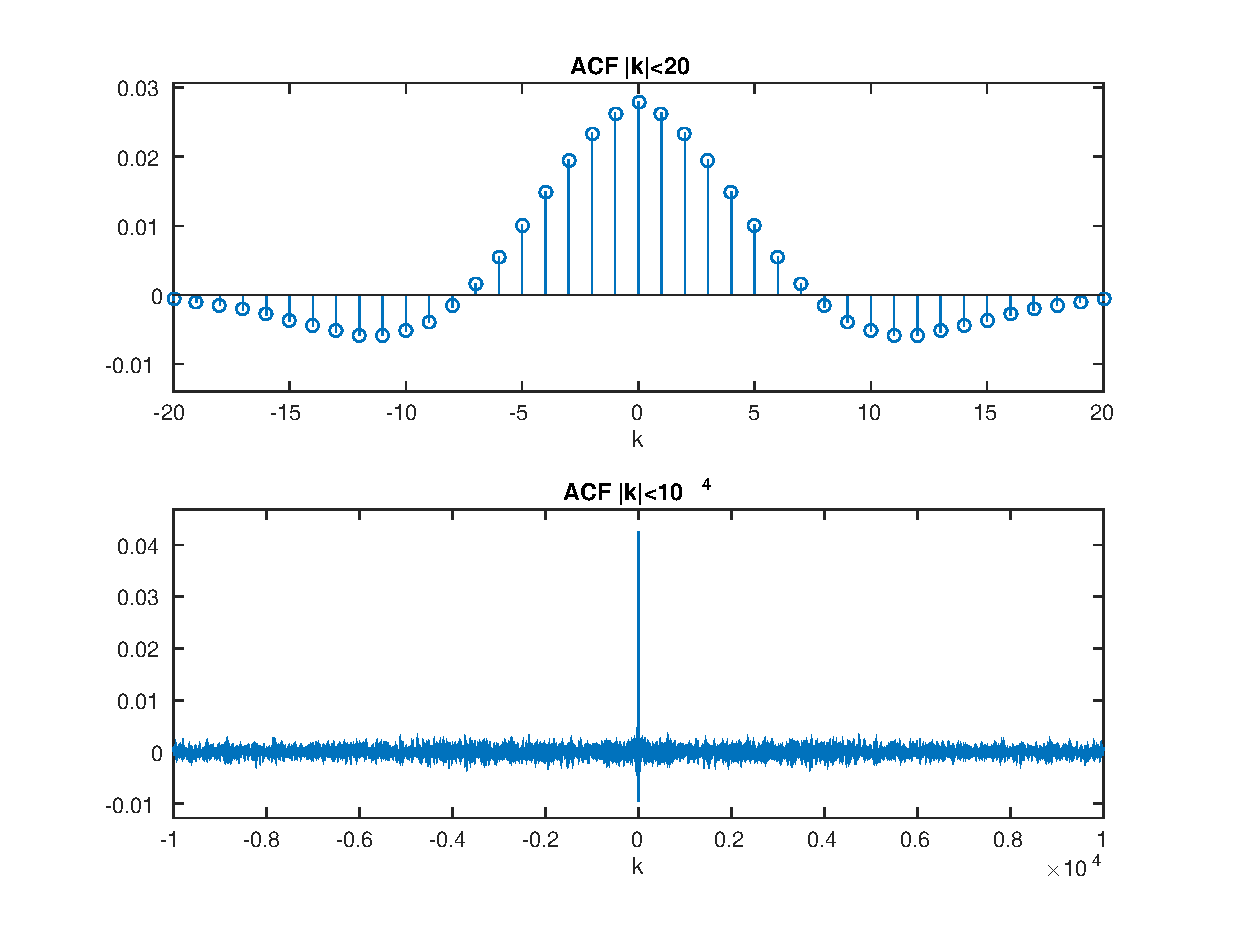
\includegraphics[width=0.8\textwidth]{bilder/Lab1/Lab1fig4.eps}
\caption{High-order low-pass ACF estimate.}
\label{fig:Lab1fig4}
\end{figure}

\begin{figure}[h]
\centering
\includegraphics[width=0.8\textwidth]{bilder/Lab1/Lab1fig5.eps}
\caption{First-order low-pass PSD estimate.}
\label{fig:Lab1fig5}
\end{figure}

\begin{figure}[h]
\centering
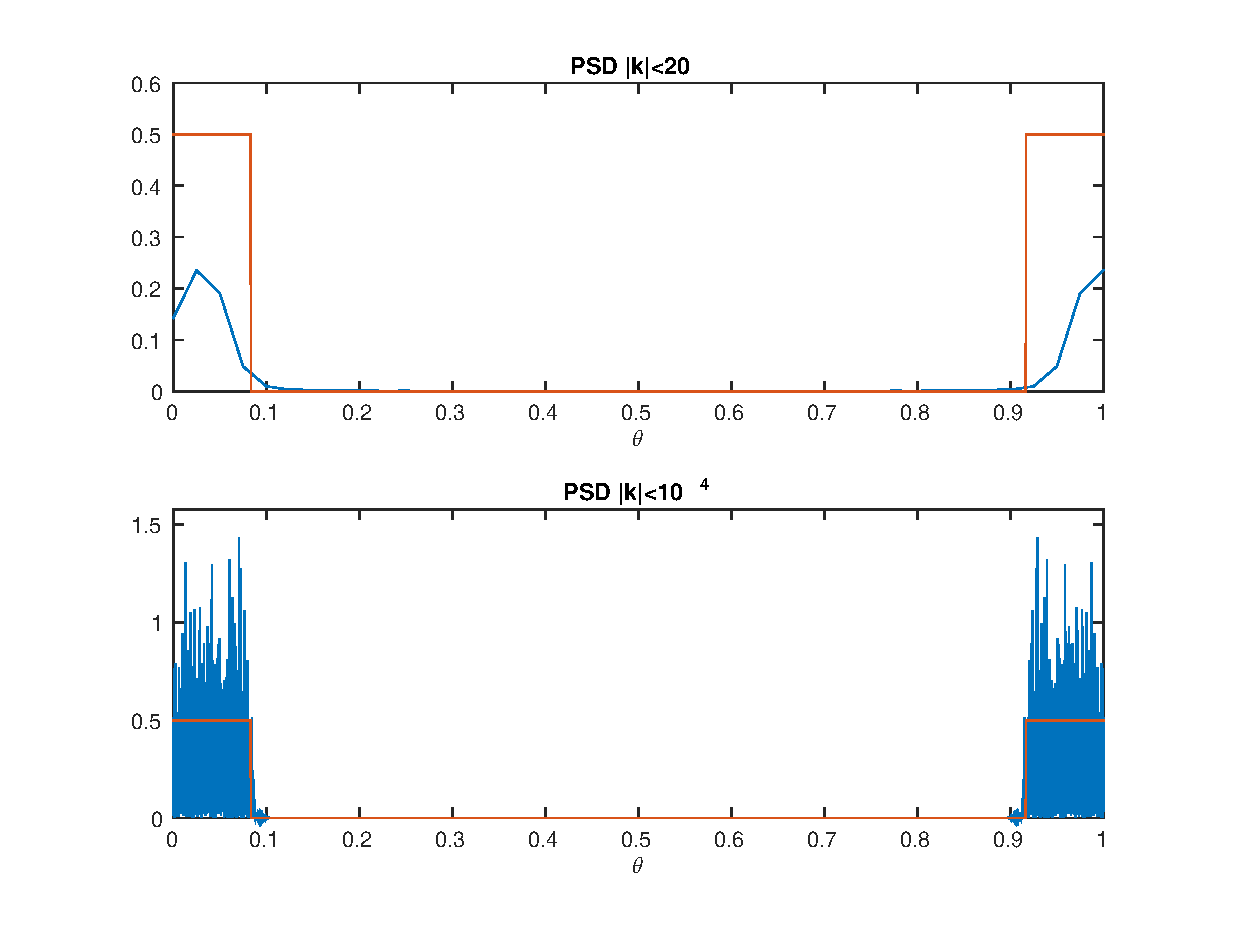
\includegraphics[width=0.8\textwidth]{bilder/Lab1/Lab1fig6.eps}
\caption{High-order low-pass PSD estimate.}
\label{fig:Lab1fig6}
\end{figure}


%%%%%%%%%%%%%%%%% Improved estimations %%%%%%%%%%%%%%%%%%%%

\subsection{Improved estimations}


%%%%%%%%%%%%%%%%% Bartletts %%%%%%%%%%%%%%%%%%%%%%%%%%%%%%%

\subsubsection{Avering periodograms}

\begin{figure}[h]
\centering
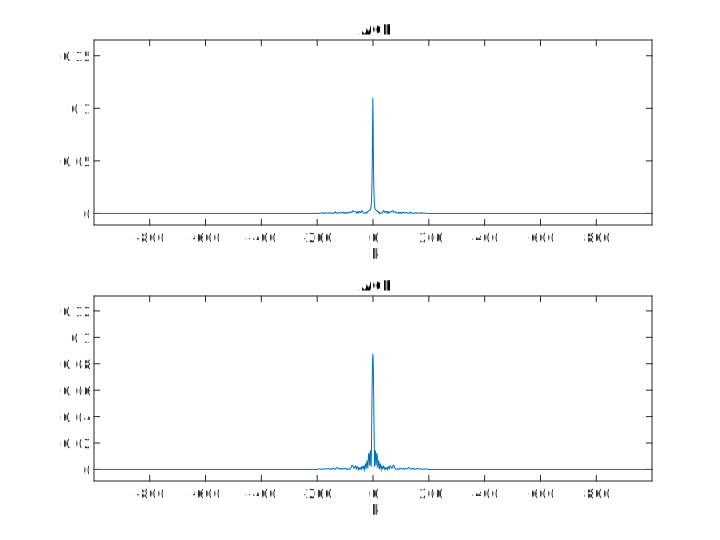
\includegraphics[width=0.8\textwidth]{bilder/Lab1/Lab1fig8.eps}
\caption{Low-order low-pass PSD and ACF improved estimates.}
\label{fig:Lab1fig8}
\end{figure}

\begin{figure}[h]
\centering
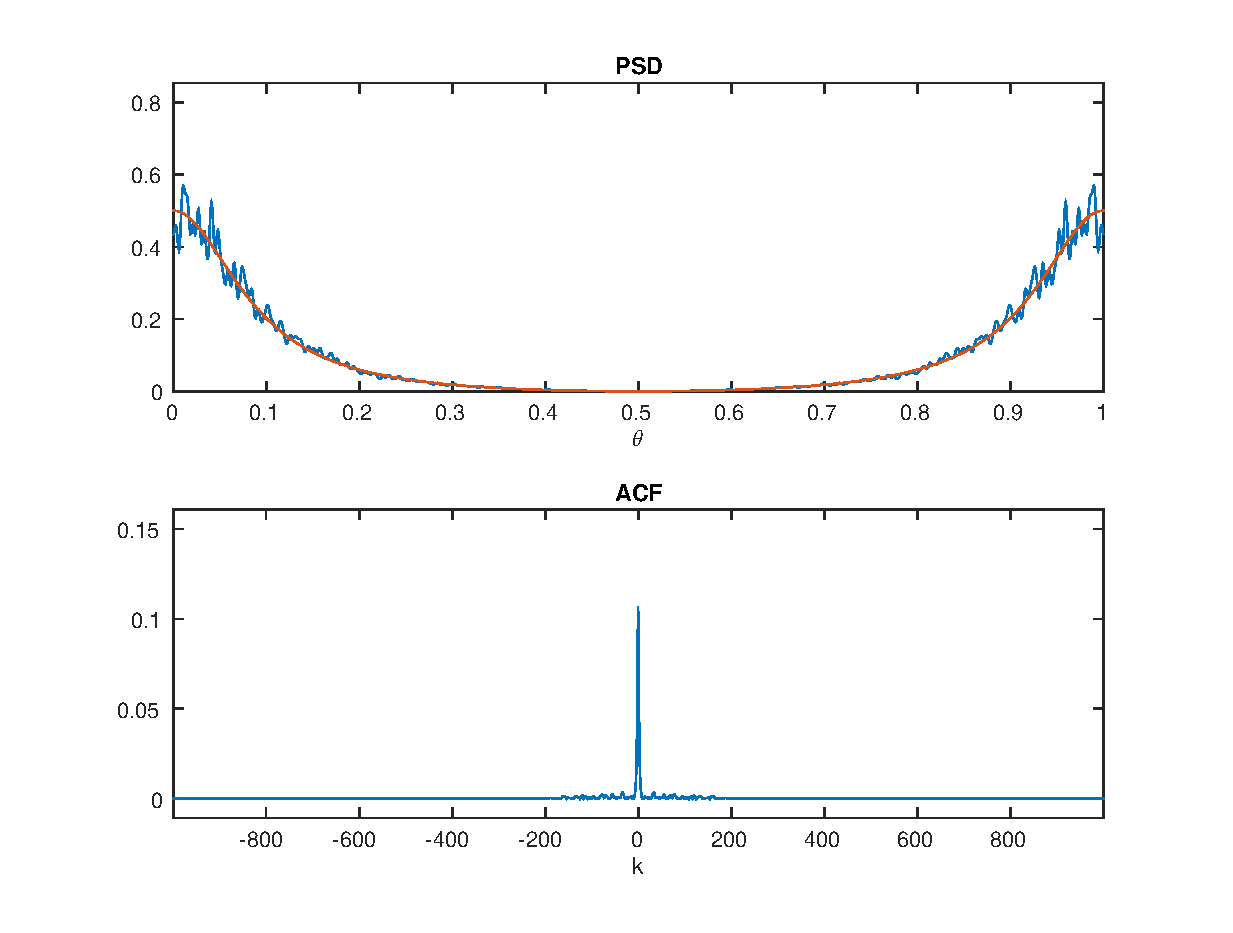
\includegraphics[width=0.8\textwidth]{bilder/Lab1/Lab1fig7.eps}
\caption{High-order low-pass PSD and ACF improved estimates.}
\label{fig:Lab1fig7}
\end{figure}


%%%%%%%%%%%%%%%%% Bartletts %%%%%%%%%%%%%%%%%%%%%%%%%%%%%%%

\subsubsection{Smoothing}

\begin{figure}[h]
\centering
\includegraphics[width=0.8\textwidth]{bilder/Lab1/Lab1fig11.eps}
\caption{Some diffrent windows used in smoothing.}
\label{fig:Lab1fig11}
\end{figure}

\begin{figure}[h]
\centering
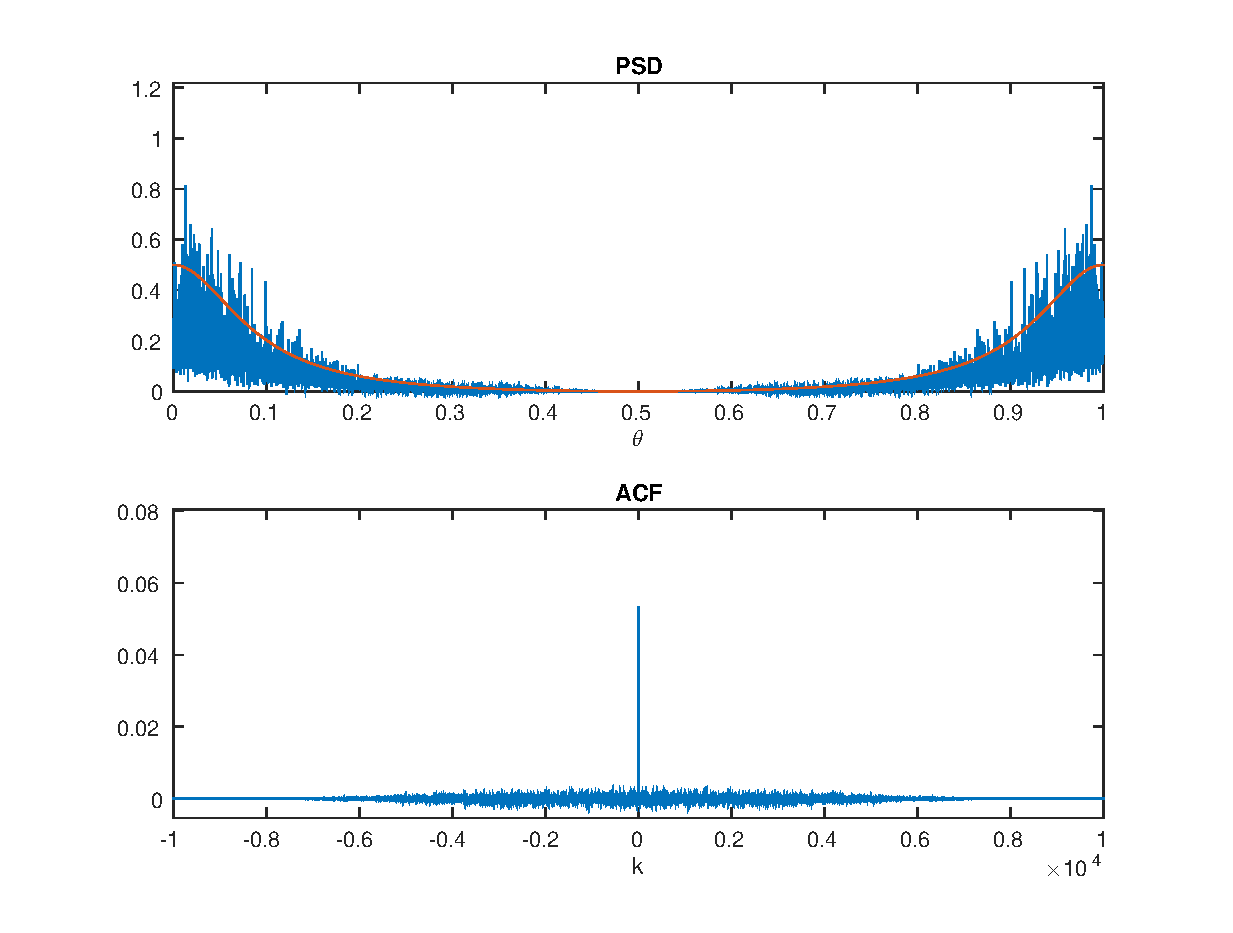
\includegraphics[width=0.8\textwidth]{bilder/Lab1/Lab1fig9.eps}
\caption{Low-order low-pass ACF and PSD improved estimate.}
\label{fig:Lab1fig9}
\end{figure}

\begin{figure}[h]
\centering
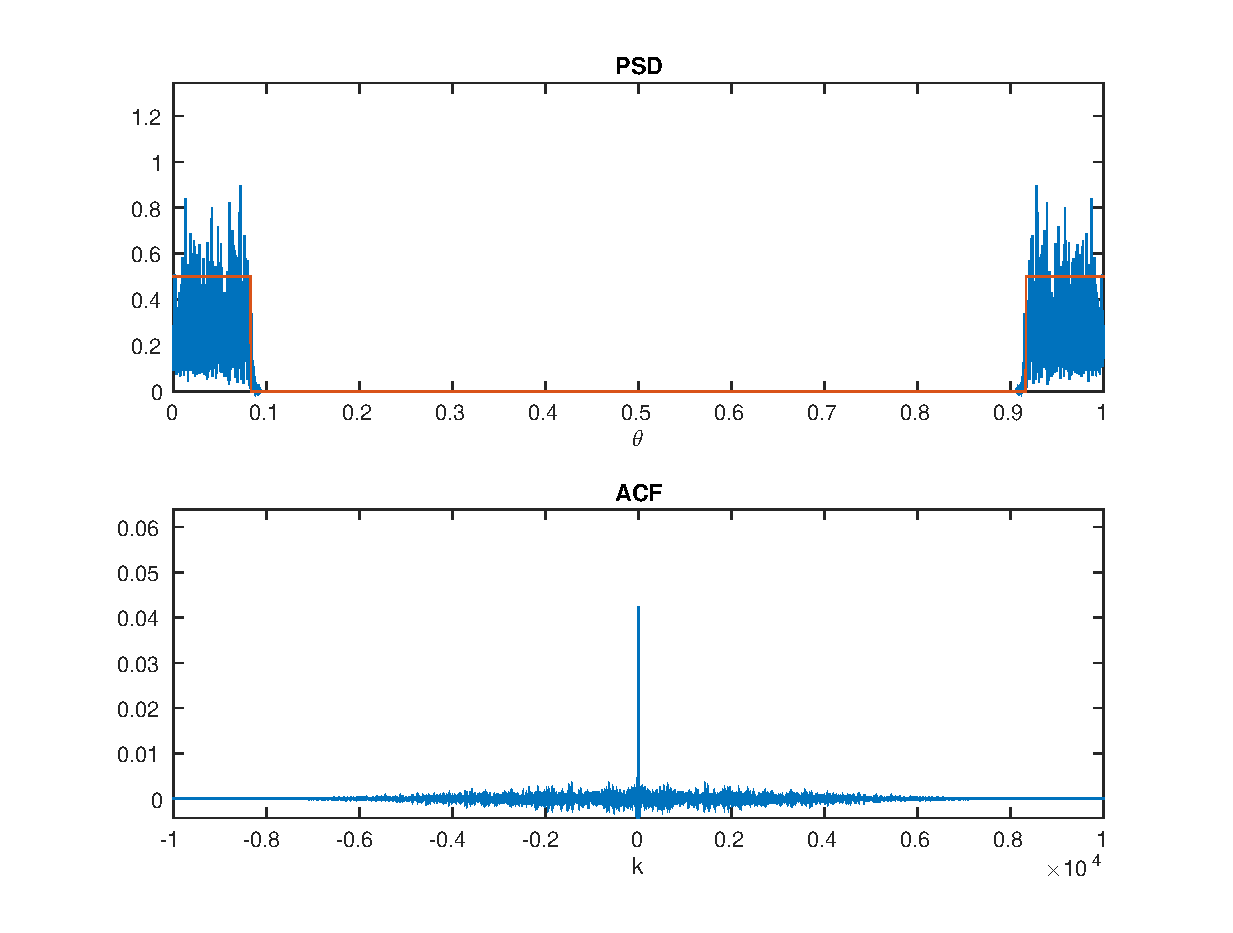
\includegraphics[width=0.8\textwidth]{bilder/Lab1/Lab1fig10.eps}
\caption{High-order low-pass ACF and PSD improved estimate.}
\label{fig:Lab1fig10}
\end{figure}


%%%%%%%%%%%%%%%%% Discussion %%%%%%%%%%%%%%%%%%%%%%%%%%%%%%

\subsection{Discussion}


%%%%%%%%%%%%%%%%%%%%%%%%%%%%%%%%%%%%%%%%%%%%%%%%%%%%%%%%%%%
%%%%%%%%%%%%%%%%% Study 2 - Non-LTI-systems %%%%%%%%%%%%%%%
%%%%%%%%%%%%%%%%%%%%%%%%%%%%%%%%%%%%%%%%%%%%%%%%%%%%%%%%%%%

\section{Study 2 - Non-LTI-systems}


%%%%%%%%%%%%%%%%% Theoretical calculations %%%%%%%%%%%%%%%%

\subsection{Theoretical calculations}

\subsubsection{Squarer}

\begin{figure}[h]
\centering
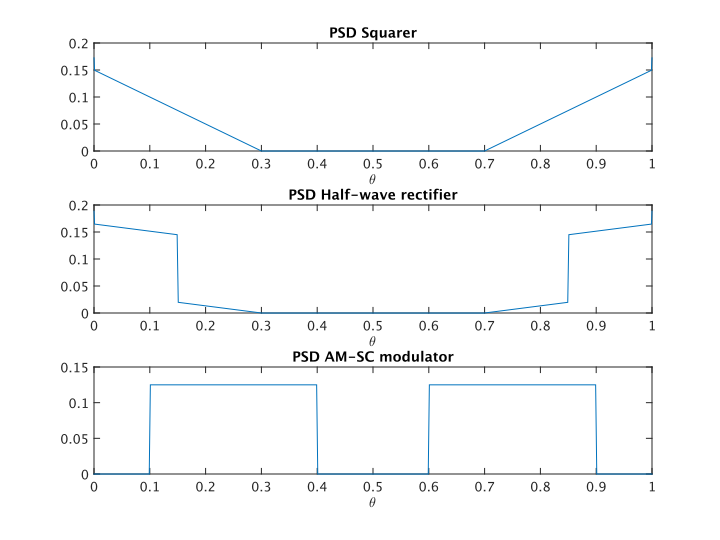
\includegraphics[width=0.8\textwidth]{bilder/Lab2/Lab2fig1.eps}
\caption{PSD and ACF of first-order low-pass filter.}
\label{fig:Lab2fig1}
\end{figure}

\subsubsection{Half-wave rectifier}

\begin{figure}[h]
\centering
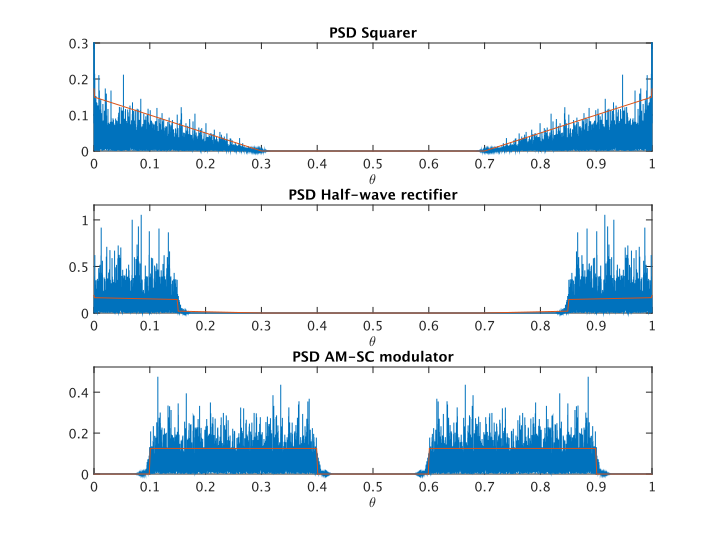
\includegraphics[width=0.8\textwidth]{bilder/Lab2/Lab2fig2.eps}
\caption{PSD and ACF of first-order low-pass filter.}
\label{fig:Lab1fig1}
\end{figure}

\subsubsection{AM-SC modulator}

\begin{figure}[h]
\centering
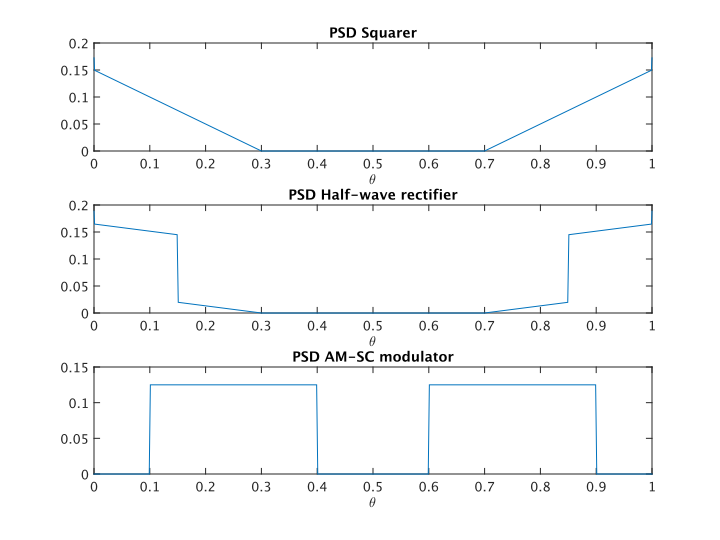
\includegraphics[width=0.8\textwidth]{bilder/Lab2/Lab2fig1.eps}
\caption{PSD and ACF of first-order low-pass filter.}
\label{fig:Lab1fig1}
\end{figure}

%%%%%%%%%%%%%%%%% Estimations %%%%%%%%%%%%%%%%%%%%%%%%%%%%%

\subsection{Estimations}

\subsubsection{Bartletts}
\begin{figure}[h]
\centering
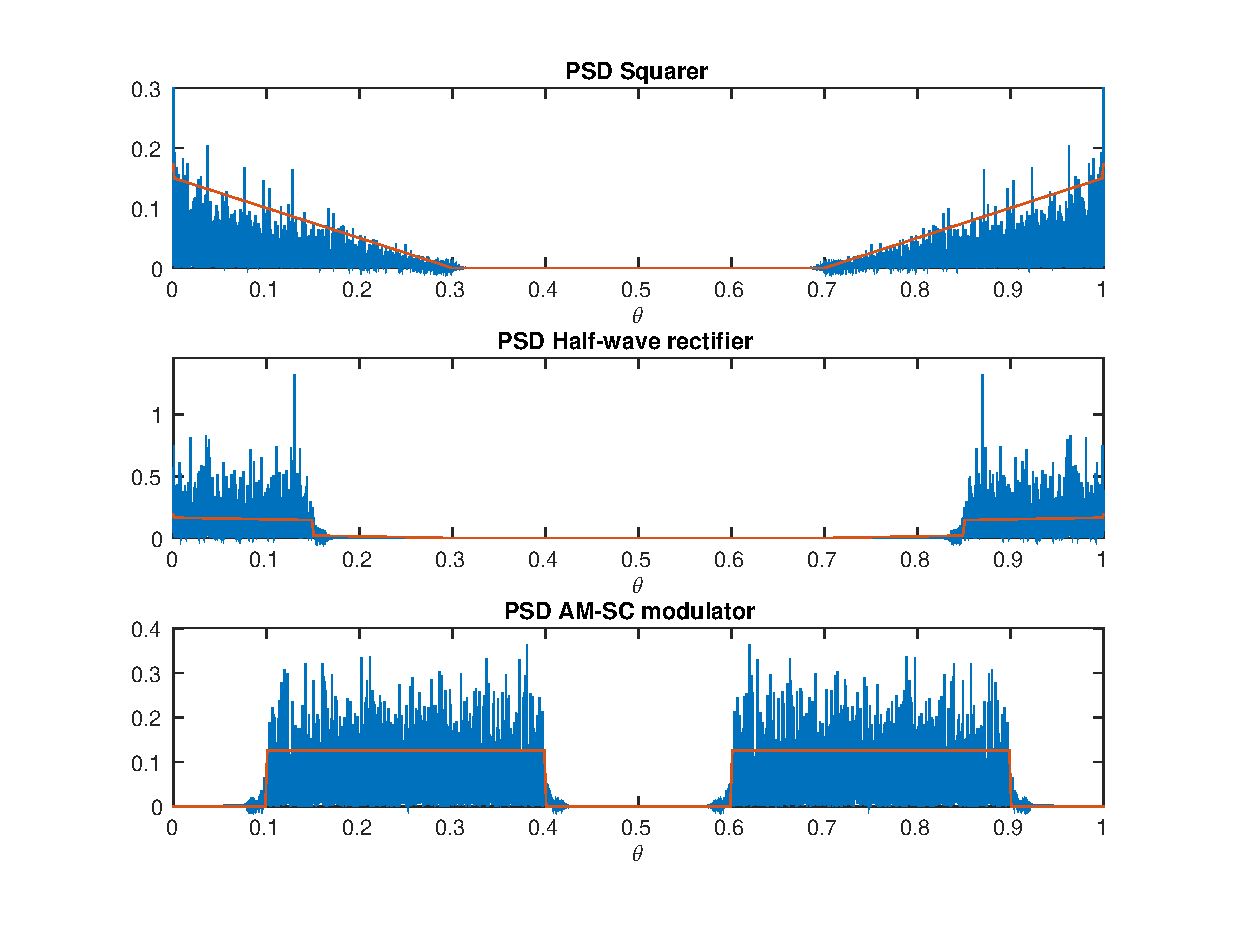
\includegraphics[width=0.8\textwidth]{bilder/Lab2/Lab2fig7.eps}
\caption{PSD and ACF of first-order low-pass filter.}
\label{fig:Lab1fig1}
\end{figure}

%%%%%%%%%%%%%%%%% Improved estimations %%%%%%%%%%%%%%%%%%%%

\subsection{Improved estimations}


\subsubsection{Avering periodograms}
\begin{figure}[h]
\centering
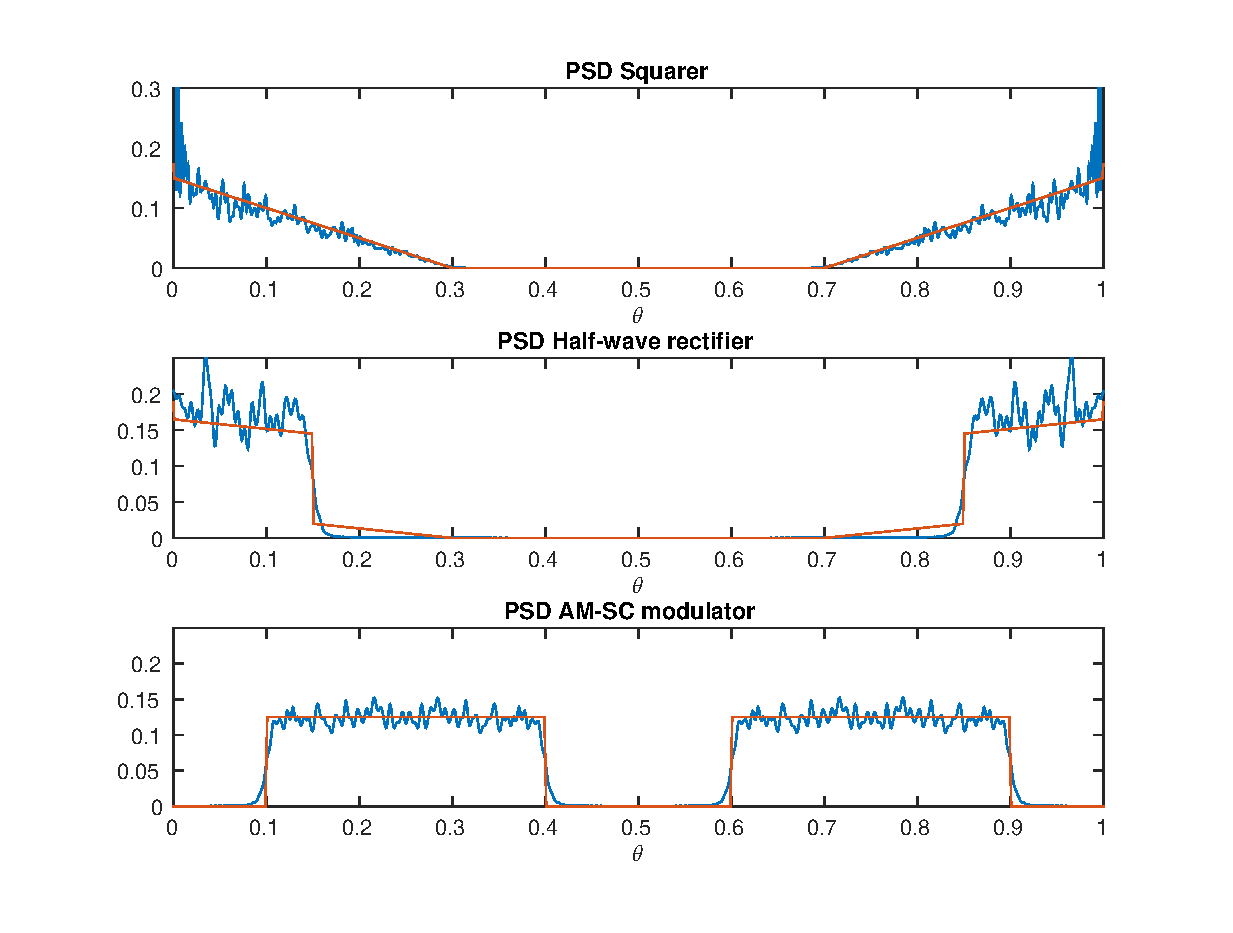
\includegraphics[width=0.8\textwidth]{bilder/Lab2/Lab2fig8.eps}
\caption{PSD and ACF of first-order low-pass filter.}
\label{fig:Lab1fig1}
\end{figure}

\subsubsection{Smoothing}
\begin{figure}[h]
\centering
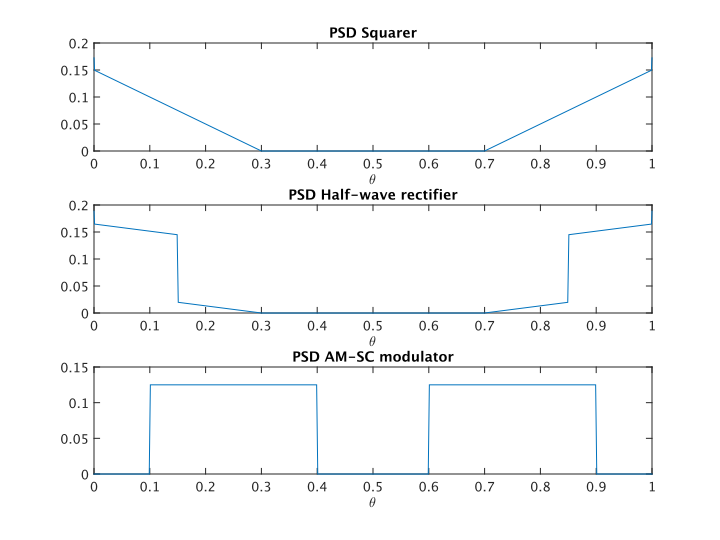
\includegraphics[width=0.8\textwidth]{bilder/Lab2/Lab2fig1.eps}
\caption{PSD and ACF of first-order low-pass filter.}
\label{fig:Lab1fig1}
\end{figure}

%%%%%%%%%%%%%%%%% Discussion %%%%%%%%%%%%%%%%%%%%%%%%%%%%%%

\subsection{Histogram}


%%%%%%%%%%%%%%%%% Discussion %%%%%%%%%%%%%%%%%%%%%%%%%%%%%%

\subsection{Discussion}

%%%%%%%%%%%%%%%%%%%%%%%%%%%%%%%%%%%%%%%%%%%%%%%%%%%%%%%%%%%
%%%%%%%%%%%%%%%%% Study 3 - Special Operations %%%%%%%%%%%%
%%%%%%%%%%%%%%%%%%%%%%%%%%%%%%%%%%%%%%%%%%%%%%%%%%%%%%%%%%%

\section{Study 3 - Special Operations}

%%%%%%%%%%%%%%%%% Theoretical calculations %%%%%%%%%%%%%%%%

\subsection{Theoretical calculations}

%%%%%%%%%%%%%%%%% Alternator %%%%%%%%%%%%%%%%%%%%%%%%%%%%%%

\subsubsection{Alternator}

%%%%%%%%%%%%%%%%% Decimator %%%%%%%%%%%%%%%%%%%%%%%%%%%%%%%

\subsubsection{Decimator}

%%%%%%%%%%%%%%%%% Estimations %%%%%%%%%%%%%%%%%%%%%%%%%%%%%

\subsection{Estimations}

%%%%%%%%%%%%%%%%% Bartletts %%%%%%%%%%%%%%%%%%%%%%%%%%%%%%%

\subsubsection{Bartletts}

%%%%%%%%%%%%%%%%% Improved estimations %%%%%%%%%%%%%%%%%%%%

\subsection{Improved estimations}

%%%%%%%%%%%%%%%%% Avering periodograms %%%%%%%%%%%%%%%%%%%%

\subsubsection{Avering periodograms}

%%%%%%%%%%%%%%%%% Discussion %%%%%%%%%%%%%%%%%%%%%%%%%%%%%%

\subsection{Discussion}

\end{document}
